\documentclass[a4paper,11pt]{article}
\usepackage[utf8]{inputenc}
\usepackage{enumitem}
\usepackage{setspace}
\usepackage[T1]{fontenc}
\usepackage{tgtermes}
\usepackage{geometry}
\usepackage{graphicx}


 \geometry{
 a4paper,
 total={210mm,297mm},
 left=10mm,
 right=10mm,
 top=10mm,
 bottom=10mm,
  }
\NeedsTeXFormat{LaTeX2e}
\ProvidesClass{proposalnsf}[2008/06/01 NSF proposal style v1.3 SGLS]
\DeclareOption*{\PassOptionsToClass{\CurrentOption}{article}}
\ProcessOptions
\RequirePackage{calc}
%\RequirePackage{pdffig}
\RequirePackage{natbib}
\RequirePackage[american]{babel}
%\RequirePackage{hyperref}
\RequirePackage{mathpazo}
%\RequirePackage{newcent}
\setlength{\paperheight}{11in}
\setlength{\paperwidth}{8.5in}
\addtolength{\voffset}{-1in}
\addtolength{\hoffset}{-1in}
\setlength{\topmargin}{1in}
\setlength{\oddsidemargin}{1in}
\setlength{\evensidemargin}{1in}
\setlength{\textwidth}{\paperwidth - 2in}
\setlength{\textheight}{\paperheight - 2in}
\setlength{\footskip}{36pt}
\setlength{\marginparsep}{0.5cm}
\setlength{\marginparwidth}{1.5cm}
\setlength{\headheight}{0pt}
\setlength{\headsep}{0pt}
\RequirePackage{fancyhdr}
\pagestyle{fancyplain}
\renewcommand{\headrulewidth}{0pt}
\lhead{}
\chead{}
\rhead{}
\lfoot{}
\cfoot{\thepage}
\rfoot{}
\renewcommand*{\bibfont}{\small}
\pagestyle{fancy}
\fancyhf{} % clear all header and footer fields
\fancyfoot[C]{ Page \footnotesize\thepage }
\fancyfoot[L]{\footnotesize Annual report 19-20}
\fancyfoot[R]{\footnotesize Sridhar Neelamraju}


%\def\@makefnmark{\hbox{$^{\fnsymbol{\@mpfn}}\m@th$}}
\renewcommand\floatpagefraction{.9}


%opening
\title{ \vspace{-9ex}NiC Fellowship: Annual report (2019-2020)\\\line(1,0){250}}
\date{\vspace{-11ex}}


\begin{document}

\maketitle
\section{Research highlights from first two years}
I would first like to highlight the research achievements from the  first two years of the fellowship. 
\begin{itemize}
    \item {Article on new developments in the Threshold algorithm was published in the \textit{Journal of Chemical Physics} and won an Editors' Choice award in 2017. The novel stochastic search methods outlined in the manuscript enable application of energy landscape exploration methods to complex chemical systems like proteins. This was part o the original proposal for the fellowship as Work Package 4.} 
    \item{The OPTIM-SBM interface that combines the discrete path sampling methodology developed in Cambridge and Structure Based Model expertise at NCBS was developed.  This enabled application of Discrete Path Sampling method to coarse-grained proteins as described in the original proposal for the fellowship. A proof-of-concept study comparing energy landscapes of a naturally evolved protein versus a designed protein was published in \textit{Journal of  Physical Chemistry B.}}
    \item{A new software package called Go-kit was developed from scratch to enable users employ the method developed above for any single-domain protein. The only input needed was the PDBID of the protein. This was published as open-source software in \textit{Journal of Chemical Information and Modeling}. The software was well received and slowly a user base appears to be building.}
    In the next section, I will outline new developments since moving to Cambridge in January, 2019

\end{itemize}
\section{Work performed over the past year (Since Jan, 2019)}
\subsection{Quasi-Continuous Interpolation scheme coupled to Structure Based Models (QCI-SBM)} 
Over the first six months in Cambridge, I enhaced the OPTIM-SBM interface by adding Quasi-Continuous Interpolations to it. This enhancement in methodology now enables the study of proteins with complex topologies that are not amenable to typical computational chemistry methods like molecular dynamics. Further, with the help of the group at Cambridge, I was able to apply to my problem, a graph traversal algorithm that found distinct paths connecting any two nodes on a disconnectivity graph. As described in the original proposal, a disconnectivity graph is how we represent our database of hundreds of thousands of connected stationary points found for a given protein. In this manner, we are able to find multiple paths connecting any two protein conformations (described as local minima, or, nodes on the disconnectivity graph). 

We tested the methodology on proteins that form complex knots and are difficult to fold.
\subsection{Application to a model trefoil knot}
A trefoil knot is the simplest non-trivial knot. The simplest protein that folds into this topology comprises only 92 amino acids (PDB:2EFV). The QCI-SBM  method was applied to this protein to see if results known from literature were reproducible. Not only were we able to reproduce known results, but we added significantly to the understanding of the energy landscape of this simple trefoil knotted protein in many ways. Some results in Figures \ref{fig:2efv_1} and \ref{fig:2efv_2}
\begin{figure}[htbp]
    \centering
    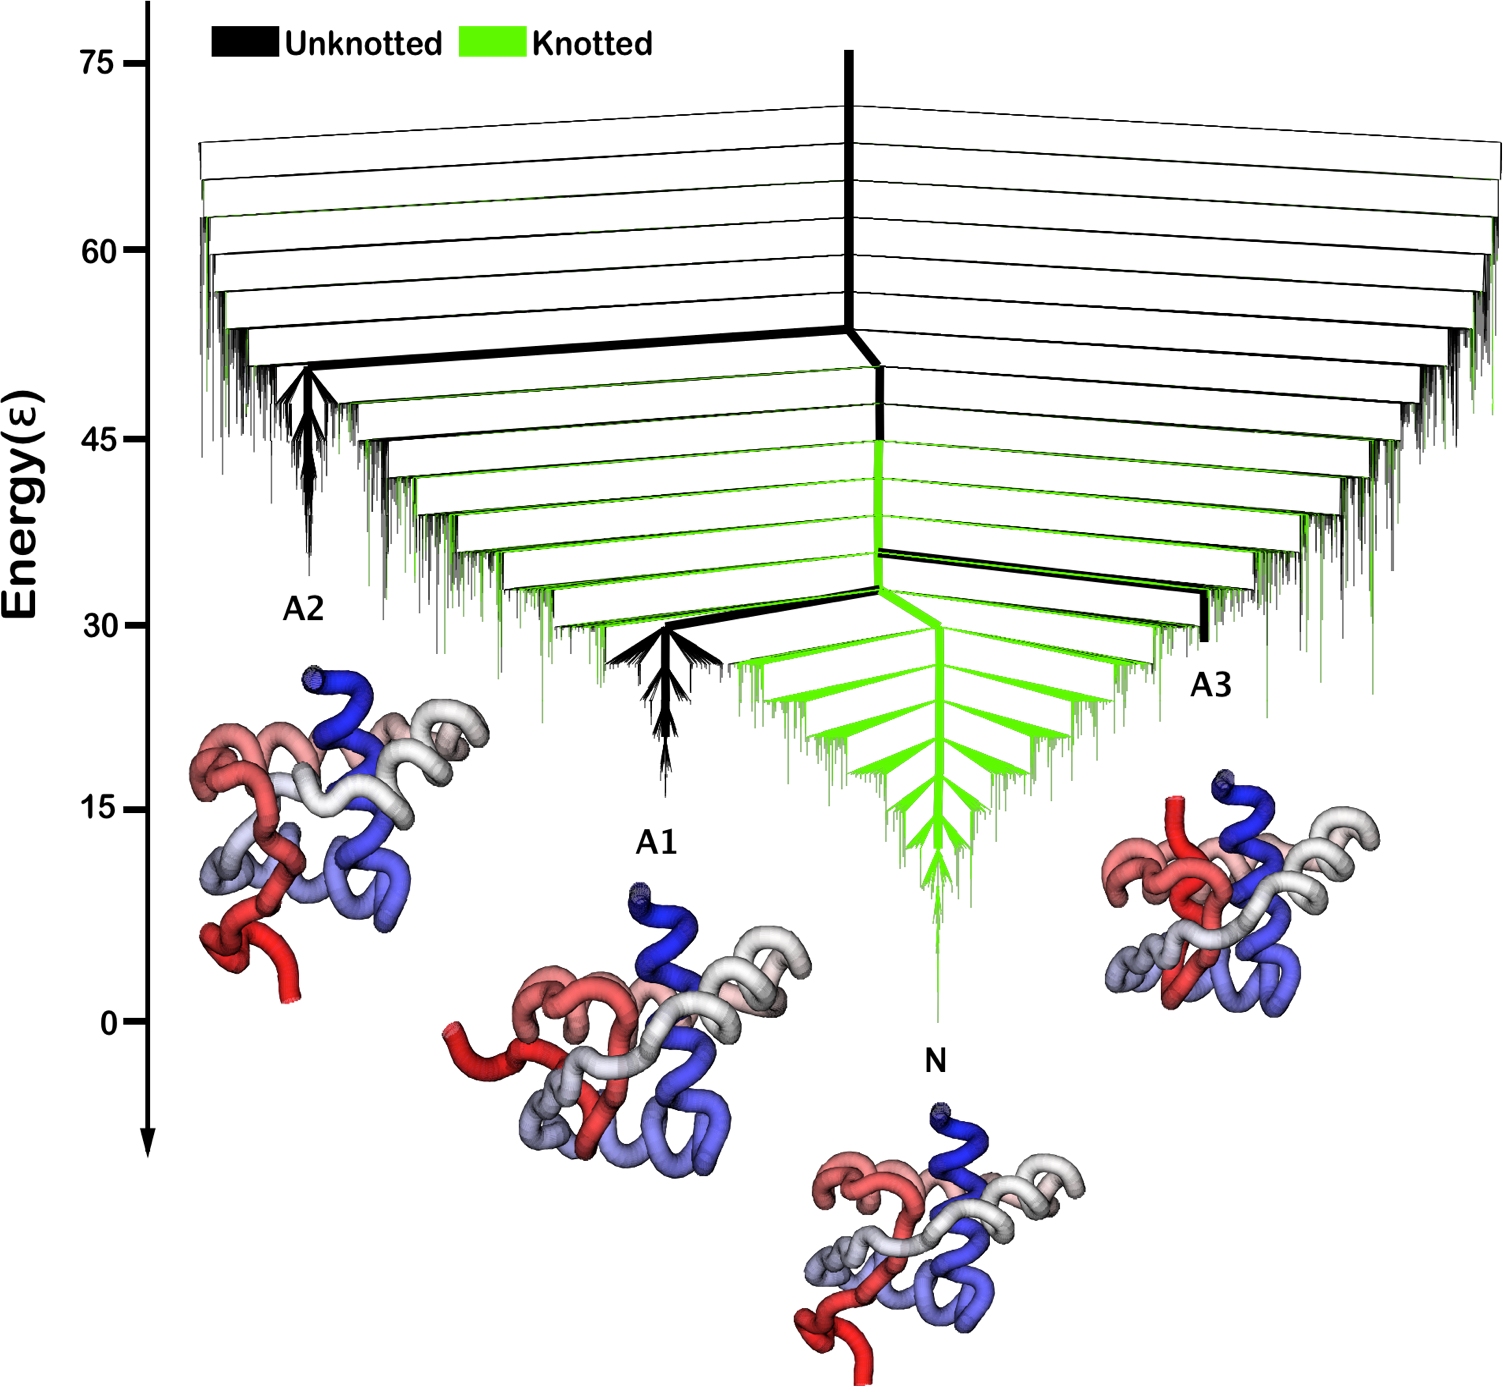
\includegraphics[height=4cm]{2efv_mukund.png}
    \caption{Disconnectivity graph for a protein that forms a simple shallow trefoil knot. Green nodes are local minima with a knotted topology while black nodes are local minima with an unknotted topology.}
    \label{fig:2efv_1}
\end{figure}
\begin{figure}[htbp]
    \centering
    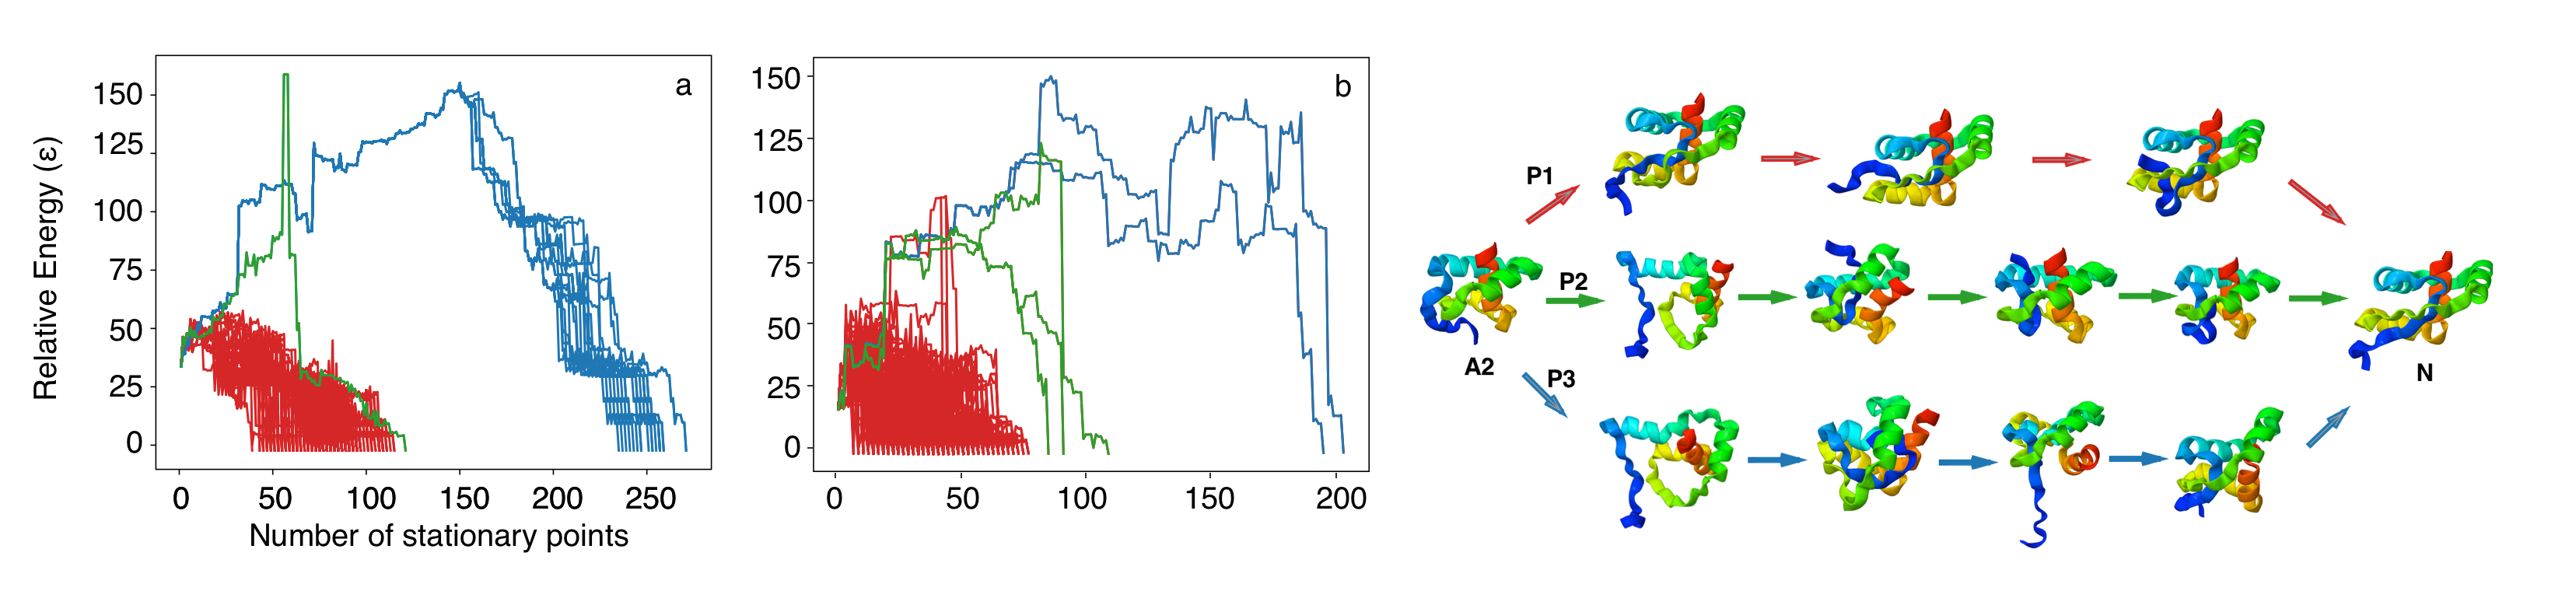
\includegraphics[height=4cm]{2efv_mukund2.png}
    \caption{Left: Distinct paths separating two topological traps found on the energy landscape of a protein that forms a model trefoil knot derived from the disconnectivity graph  shown above. Colour indicates representative physically distinct mechanisms Right: Pictorial depiction of the three representative pathways  found from topological trap A2 to the native knotted topology. }
    \label{fig:2efv_2}
\end{figure}

\subsection{Application to a deep trefoil knot}
A deep trefoil knot is a particularly hard protein to fold with molecular dynamics (PDBID:1mxi). Previous studies had a 0\% success rate of finding the native-state of this protein with the C$\alpha$ model description. We show that with QCI-SBM, this challenging protein can also be folded. In fact, we find multiple pathways with which a deep trefoil knot can form. The most thermodynamically favourable pathway includes very interesting combination of loop-flipping and slip-knotting moves that have not yet been reported in literature. Some example results in Figures \ref{fig:mxi20_1} and \ref{fig:mxi20_2}. An article describing these results has been drafted and will be submitted soon. 
\begin{figure}[htbp]
    \centering
    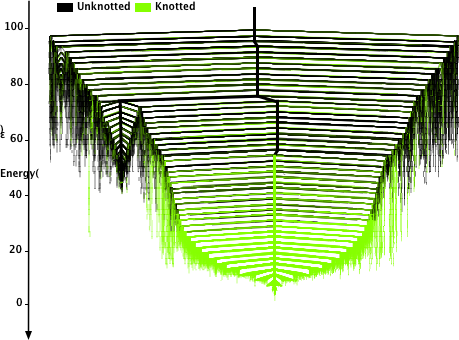
\includegraphics[height=4cm]{1mxi20.png}
    \caption{Disconnectivity graph for a protein that forms a deep trefoil knot. The sub-funnel corresponds to the jammed slip-knotted intermediate showed in Figure 4 (right) while lowest energy node corresponds to the native deep-knotted state.}
    \label{fig:mxi20_1}
\end{figure}

\begin{figure}[htbp]
    \centering
    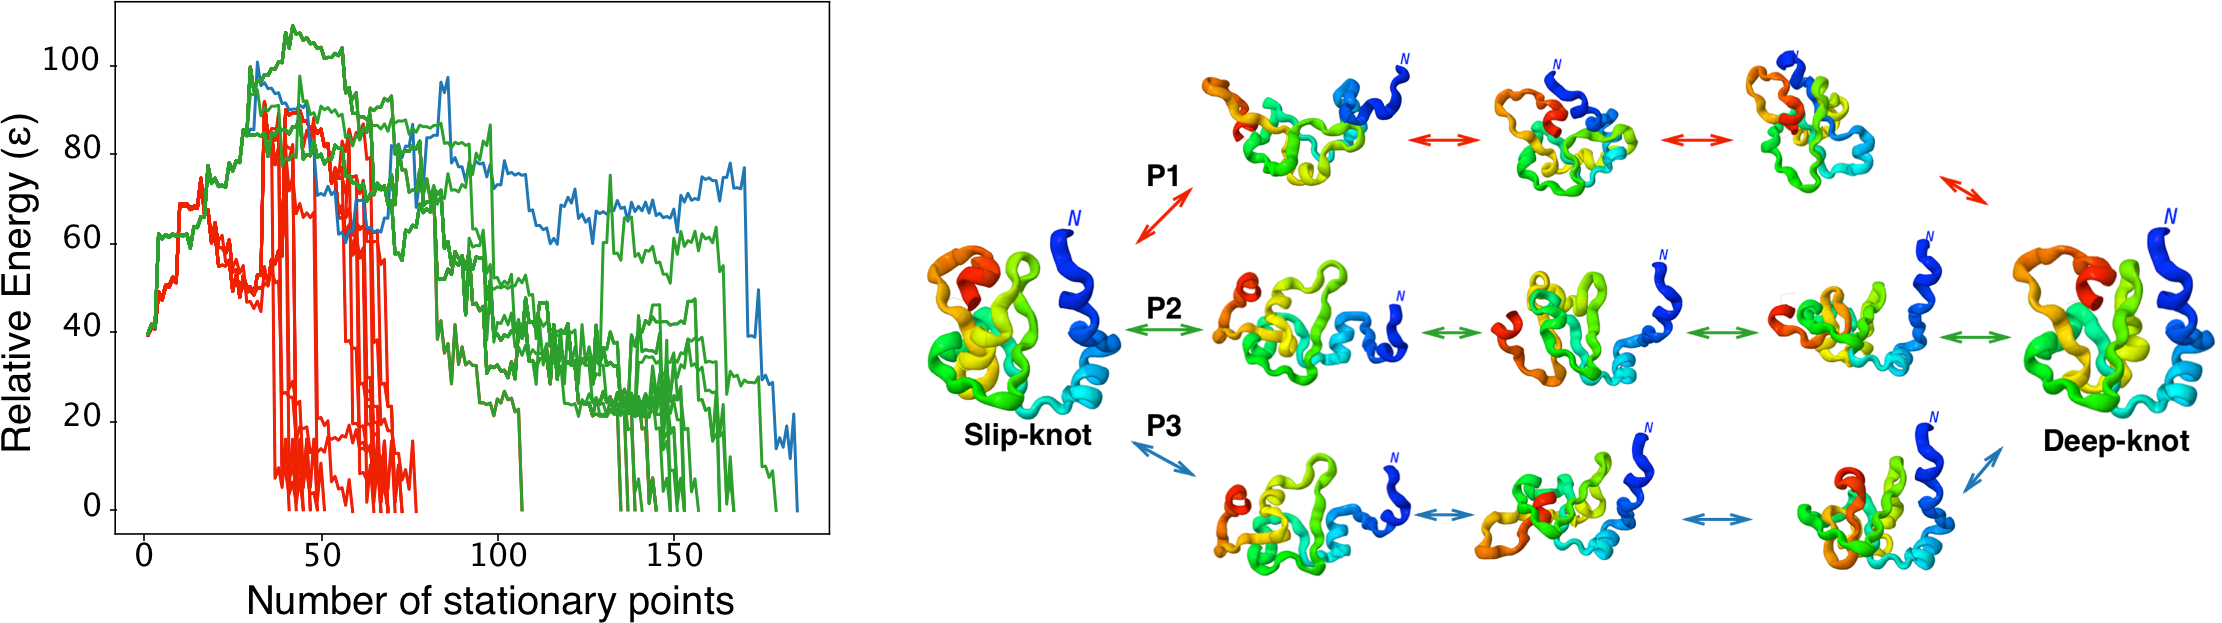
\includegraphics[height=4cm]{1mxi20_kdfig.png}
    \caption{Multiple pathways to convert a slip-knotted intermediate state to a deep trefoil knotted state derived from the disconnectivity graph. Colour scheme identical to Figure 2. P1, the shortest thermodynamic path, has never been reported in literature.}
    \label{fig:mxi20_2}
\end{figure}

\subsection{Application to a Gordian knot}
An even more challenging case is the Gordian knot. Proteins exist in nature that fold into this complex topology. I have now been able to find at least two distinct pathways with which a protein can fold into such a complex topology with the novel QCI-SBM methodology. This work is in its infancy and will take a few months to really understand the nature of the energy landscape of this complex protein.
\section{Further possibilities}
In 2016, a completely new class of proteins called entangled proteins were discovered. These included proteins that folded into knots, slip-knots, links and lassos. Folding behaviour of entangled proteins is not at all well understood. The QCI-SBM method is very well-suited for the study of these proteins. Most entangled proteins are not as intricately folded as a Gordian knot. So, a Gordian knot is a very thorough test of the QCI-SBM methodology that allows its application to all types of entangled proteins in the future. This should open up a whole new way of studying energy landscapes of complex proteins. 
\section{Applications for new positions}
I'm now in the process of applying for assistant professor positions in the UK and in India. I just interviewed at IIT-Madras and am awaiting a decision. I also have applications pending at Ashoka University, KREA University and Aarhus University (Denmark). I have also been suggested as a candidate for holding a University Research Fellowship (Tenure-track) at the University of Nottingham, UK. I would be glad if NCBS could consider extending the NiC fellowship support at Cambridge for three or four more months beyond January, 2020. I could use this time to interview for the University Research Fellowship position at Nottingham and other European/British universities as well.  
\bibliography{knots}
\bibliographystyle{unsrt}
\end{document}